\documentclass[mathserif]{beamer}%Agregar ,notes antes del ] para incluir las notas.
%~ \documentclass[handout]{beamer}

% Tema (colores, bordes, secciones, etc)
\usetheme{Warsaw}

% Configuracion del tema
\setbeamertemplate{navigation symbols}{} % saca los simbolos de abajo a la derecha
\useoutertheme{infolines} % muestra datos abajo de todo (nombre, numero de slide, etc)
\usecolortheme[RGB={72,123,127}]{structure}

% Paquetes usados
\usepackage[utf8]{inputenc}
\usepackage[spanish, es-tabla]{babel}
\usepackage{indentfirst}
\usepackage{beamerthemeshadow}
\usepackage{xspace}
\usepackage{latexsym}
\usepackage{ulem}
\usepackage{color}
\usepackage{tikz}
\usepackage{pgfplots}
\usepackage{colortbl, xcolor}
\usepackage{longtable}
\usepackage{graphicx}
\usepackage{wrapfig}
\usepackage{multicol}
\usepackage{multirow}

\usepackage{etex}
\usepackage{dirtree}

\usepackage{tikz}
\usepackage{pgfplots}
\pgfplotsset{width=15cm, height=8cm}

%definicion para grafico en analisis de fold
\usetikzlibrary{shapes.geometric, arrows}

\tikzstyle{datos} = [rectangle, rounded corners, minimum width=12cm, minimum height=1cm,text centered, draw=black, fill=red!30]
\tikzstyle{train} = [rectangle, rounded corners, minimum width=2cm, minimum height=1cm,text centered, draw=black, fill=red!30]
\tikzstyle{test} = [rectangle, minimum width=2cm, minimum height=0.5cm, text centered, draw=black, fill=orange!30]
\tikzstyle{prom} = [rectangle, rounded corners, minimum width=8cm, minimum height=0.5cm, text centered, draw=black, fill=blue!30]
\tikzstyle{fold} = [rectangle, minimum width=2cm, minimum height=0.5cm, text centered]
\tikzstyle{proc} = [trapezium, trapezium left angle=70, trapezium right angle=110, minimum width=2cm, minimum height=0.8cm, text centered, text width=2cm, draw=black, fill=blue!30]

\tikzstyle{arrow} = [thick,->,>=stealth]
\tikzstyle{arrowBig} = [line width=8pt,->,>=stealth]

%fin fold

%definicion otros x validations
\usetikzlibrary{shapes.geometric}
\tikzset{myshade/.style={minimum size=.4cm,shading=radial,inner color=white,outer color={#1!90!gray}}}
\newcommand\mycirc[1][]{\tikz\node[circle,myshade=#1]{};}


\graphicspath{ {Images/} }

\newcommand{\tab}[1]{\hspace{.12\textwidth}\rlap{#1}}

\parskip=1ex

\title{Recolección online de grabaciones para el estudio de las variantes argentinas del español}
\author{Fernando Bugni}
\institute{Departamento de Computación - FCEyN - UBA}
\date{Fecha}
\newcommand{\director}{Directores:\\ Agustín Gravano, \\ Miguel Martínez Soler}

\setbeamertemplate{title page}{
	\centering
	\begin{beamercolorbox}[rounded=true,shadow=true,sep=8pt,center]{title}
		\inserttitle \par
	\end{beamercolorbox}
	\vfill
	\begin{beamercolorbox}[leftskip=8cm,center,wd=0.7\textwidth]{author}
		\begin{columns}[T]
			\begin{column}{.49\textwidth}%
				\centering
				\insertauthor
			\end{column}
			\begin{column}{.49\textwidth}%
				\centering
				\director
			\end{column}
		\end{columns}
	\end{beamercolorbox}
	\vfill
	\usebeamerfont{institute}\insertinstitute \par
	\vfill
	\centering
	\insertdate\par
	\vfill
}

\begin{document}
	
\title[Recolección online de grabaciones]{Recolección online de grabaciones para el estudio de las variantes argentinas del español}
\author[Fernando Bugni]{Fernando Bugni}
\institute[DC-FCEyN-UBA]{Departamento de Computación - Facultad de Ciencias Exactas - \\Universidad de Buenos Aires}
\date{2014}

\frame{\titlepage}

% % % % Introducción

\section{Introducción}

\newcommand{\man}[2]{
	\node[inner sep=0, scale=0.08] at (#1,#2){
\includegraphics[width=\textwidth]{man-profile.png}};
	\node[inner sep=0, scale=0.03] at (#1+0.45,#2+0.2){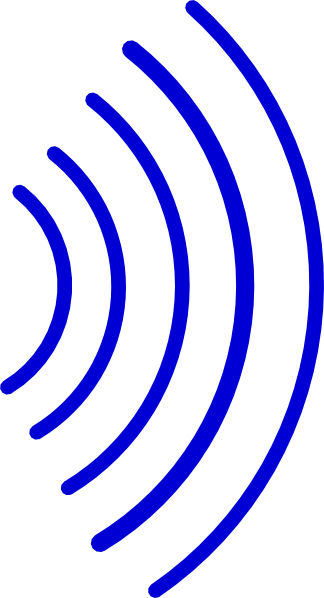
\includegraphics[width=\textwidth]{wave.png}};
}
\newcommand{\woman}[2]{
	\node[inner sep=0, scale=0.08] at (#1,#2){
\includegraphics[width=\textwidth]{woman-profile.png}};
	\node[inner sep=0, scale=0.03] at (#1+0.5,#2+0.1){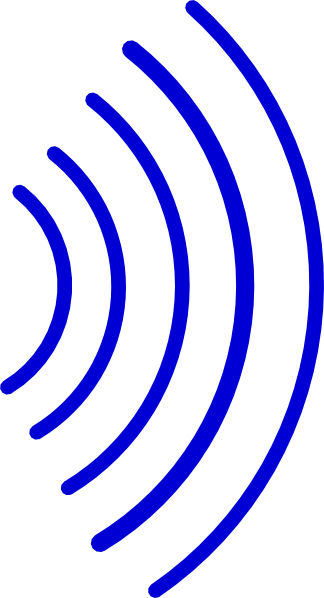
\includegraphics[width=\textwidth]{wave.png}};
}
	
\begin{frame}
	\frametitle{Recolectar grabaciones para estudios del habla}
	
	\begin{tikzpicture}
		\man{2}{0};
		\man{5}{3};
		\man{2}{6};
		\man{4}{6};
		
		\woman{1}{2};
		\woman{5}{0.5};
		\woman{3}{4};
		
		\node[inner sep=0, scale=0.1] at (11,4){
\includegraphics[width=\textwidth]{mic.jpg}};
		
	\end{tikzpicture}
\end{frame}

\def \serverpos {(11,3.5)}

\begin{frame}
	\frametitle{Recolectar grabaciones para estudios del habla}
	
	\begin{tikzpicture}
	\man{2}{0};
	\draw[dotted,thick] (2,0) -- \serverpos;
	\man{5}{3};
	\draw[dotted,thick] (5,3) -- \serverpos;
	\man{2}{6};
	\draw[dotted,thick] (2,6) -- \serverpos;
	\man{4}{6}
	\draw[dotted,thick] (4,6) -- \serverpos;
	
	\woman{1}{2};
	\draw[dotted,thick] (1,2) -- \serverpos;
	\woman{5}{0.5};
	\draw[dotted,thick] (5,0.5) -- \serverpos;
	\woman{3}{4};
	\draw[dotted,thick] (3,4) -- \serverpos;
	
	\node[inner sep=0, scale=0.2] at  \serverpos{
\includegraphics[width=\textwidth]{server.png}};
	
	\end{tikzpicture}
\end{frame}

\begin{frame}
	\frametitle{Variantes del español en Argentina}
	\begin{center}
		\begin{tikzpicture}
		\node[anchor=south west,inner sep=0] at (0,0) {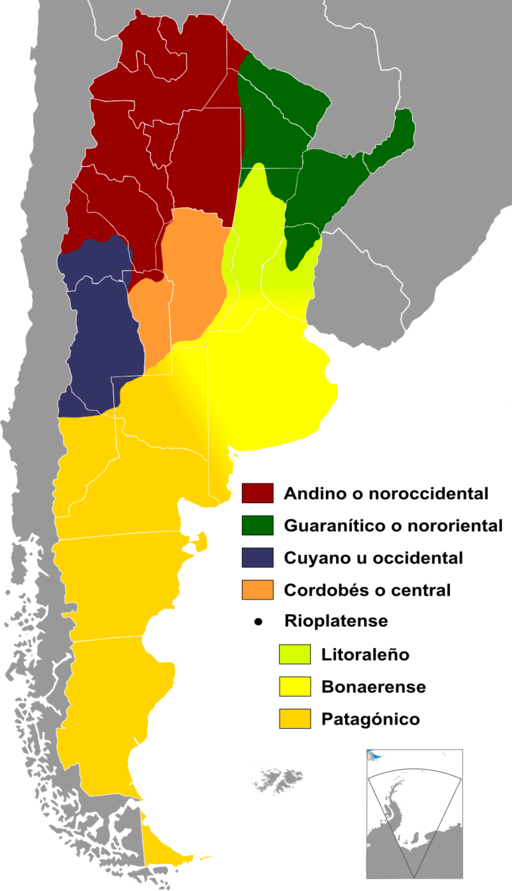
\includegraphics[scale=0.3]{../template_tesis/Images/Dialectos_del_idioma_espanol_en_Argentina.png}};
		\end{tikzpicture}
	\end{center}
\end{frame}

\begin{frame}
	\frametitle{Caso de estudio: Buenos Aires y Córdoba}
	\begin{center}
		\begin{tikzpicture}
			\node[anchor=south west,inner sep=0] at (0,0) {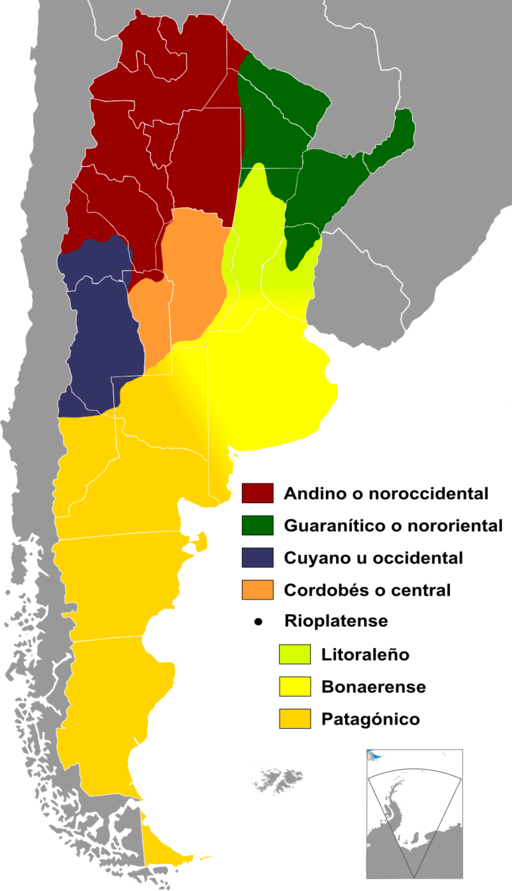
\includegraphics[scale=0.3]{../template_tesis/Images/Dialectos_del_idioma_espanol_en_Argentina.png}};
			\draw[red,ultra thick,rounded corners] (4,2.4) rectangle (2,2.7);
			\draw[red,ultra thick,rounded corners] (4,1.6) rectangle (2.3,1.9);
		\end{tikzpicture}
	\end{center}
\end{frame}

\begin{frame}
	\frametitle{Diferencias entre Córdoba y Buenos Aires}
		
	\begin{enumerate}[(1)]\itemsep=1ex
		\item Los hablantes de Córdoba estiran la sílaba anterior a la acentuada mientras los de Buenos Aires no lo hacen. Ejemplo: \textit{`Especta\textcolor{red}{\textbf{\textit{cu}}}\textcolor{blue}{lar}'} \\ 
		
		\item Los hablantes de Córdoba aspiran y elisionan la /s/ al finalizar una palabra. Esto no sucede en Buenos Aires. Ejemplo: \textit{`Pájaro\textcolor{red}{\textbf{\textit{s}}}'}\\ 
		
		\item Para hablantes de Córdoba, la /s/ antes de la /c/ o /t/ suenan más suaves que para hablantes de Buenos Aires. Ejemplo: \textit{`Mo\textcolor{red}{s}ca'} \\ 
		
		\item La `c' antes de la `t' se pronuncia con menor frecuencia para hablantes de Córdoba que para hablantes de Buenos Aires. Ejemplo: \textit{`Do\textcolor{red}{c}tor'} \\ 
		
		\item Para hablantes cordobeces la `y’ y `ll’ se pasa a `i’. No sucede esto para Buenos Aires. Ejemplo: \textit{`\textcolor{red}{ll}uvia'} \\
		
		\item En hablantes cordobeces la /r/ no vibra mientras que en Buenos Aires pasa lo contrario. Ejemplo: \textit{`Espá\textcolor{red}{rr}ago'} \\ 
	\end{enumerate}	
	
	{\tiny Bibliografía:
		\begin{itemize}
			\item El español en la Argentina y sus variedades regionales - María Beatriz Fontanella de Weinberg
			\item Español en la Argentina - Elena Vidal de Battini
		\end{itemize}}	

\end{frame}

% % % % Diseño del experimento

\section{Diseño del experimento}

\begin{frame}
	\frametitle{Diseño del experimento}
	\begin{itemize}\itemsep=10ex
		\item \textbf{Frases Comunes}: habla espontánea
		\item \textbf{Frases Amper}: reconocer palabra acentuada
	\end{itemize}	
\end{frame} 

\begin{frame}
	\frametitle{Diseño del experimento}
	{\Large Frases Comunes} \\
	Pronunciar frases popularmente conocidas
	
	\begin{itemize}
		\item Objetivo: pronunciación espontánea
		\item Reglas a cubrir: 2 a 6
	\end{itemize}

	\begin{center}
		\textbf{`En la pelea se conoce al soldado,} \\ 
		\textbf{sólo en la \textcolor{red}{victoria} se conoce al \textcolor{red}{caballero}’}
	\end{center}
	
	\begin{itemize}
		\item \textcolor{red}{\textbf{`victoria’}} cubre la \textbf{regla 4} que nos propone medir la duración de la \textit{/c/} antes de la \textit{/t/}. 
		\item \textcolor{red}{\textbf{`caballero’}} para la \textbf{regla 5} el fonema \textit{/ll/} se pasa a \textit{/i/} 
	\end{itemize}	
\end{frame} 

\begin{frame}
	\frametitle{Diseño del experimento}
	\scriptsize
	\begin{longtable}{| p{0.6\textwidth} || p{0.3\textwidth} |} 
		\hline
		\textbf{Frase} & \textbf{Frase que cubre} \\ \hline	
		
		'No hay dos sin tres' & Regla 2: 'dos', 'tres'\\ \hline
		'Más difícil que encontrar una aguja en un pajar' & Regla 2: 'más' \\ \hline
		'Más perdido que turco en la neblina' & Regla 2: 'más' \\ \hline
		'No le busques la quinta pata al gato' & Regla 2: 'busques', Regla 3: 'busques'   \\ \hline
		'Se te escapó la tortuga' & Regla 3: 'escapó'   \\ \hline
		'Todos los caminos conducen a Roma' & Regla2: 'todos', 'los', 'caminos' \\ \hline
%		'No hay mal que dure cien anos' & años &&&& \\ \hline
		'Siempre que llovió, paró' & Regla 5: llovió  \\ \hline
%		'Cría cuervos que te sacaran los ojos' & cuervos, los, ojos &&&&  \\ \hline
%		'La tercera es la vencida' & es &&&& \\ \hline
%		'Calavera no chilla' &&&& chilla &  \\ \hline
%		'La gota que rebalsó el vaso' &&&&& rebasó \\ \hline
		'La suegra y el doctor, cuanto más lejos, mejor' & Regla 2: más, lejos , Regla 4: doctor \\ \hline
%		'A la mujer picaresca cualquiera la pesca' & Regla 3:  picaresca  \\ \hline
%		'Quien siembra vientos recoge tempestades' & vientos &&&& recoge  \\ \hline
%		%	'Un grano no hace granero pero ayuda a su compañero' & \\ \hline
%		'La arquitectura es el arte de organizar el espacio' & es && arquitectura && \\ \hline
%		'El amor actúa con el corazón y no con la cabeza' &&& actúa&& \\ \hline
%		'No dudes actúa' &&& actúa&&  \\ \hline
%		%	'El niño es realista; el muchacho, idealista; el hombre, escéptico, y el viejo místico' &  \\ \hline
%		'Perro que ladra no muerde' &&&&& perro \\ \hline
%		'La musica es sinónimo de libertad, de tocar lo que quieras y como quieras' & es, quieras &&&& \\ \hline
		'La belleza que atrae, rara vez coincide con la belleza que enamora' & Regla 5: belleza  \\ \hline
		'No esta mal ser bella, lo que está mal es la obligación de serlo' & Regla 5: bella \\ \hline
%		'La batalla más difícil la tengo todos los días conmigo mismo' & más &&& batalla & \\ \hline
%		'El que no llora no mama' &&&& llora & \\ \hline
%		'En la pelea se conoce al soldado solo en la victoria se conoce al caballero' &&& victoria & caballero &\\ \hline
%		'La lectura es a la mente lo que el ejercicio al cuerpo' & es && lectura &&  \\ \hline
%		'El pez por la boca muere' & pez &&&& \\ \hline
%		'En boca cerrada no entran moscas' & moscas & moscas &&& cerrada  \\ \hline
%		'Más vale pájaro en mano que cien volando' & más &&&& \\ \hline
%		%	'La curiosidad mató al gato' &  \\ \hline
		'Río revuelto, ganancia de pescadores' & Regla 3: pescadores, Regla 2: pescadores, Regla 6: río, revuelto  \\ \hline
%		'No hay que pedirle peras al olmo' & peras &&&& \\ \hline
%		
		... & \\ \hline
		\end{longtable}
		
		\textbf{Agrega 31 Frases populares para grabar}
\end{frame}

\begin{frame}
\frametitle{Diseño del experimento}
	{\Large Frases Amper} \\
	Pronunciar frases con una estructura fija variando acentuaciones
	
	\begin{itemize}
		\item Objetivo: cubrir acentuaciones
		\item Regla a cubrir: 1
	\end{itemize}
	
{\footnotesize 	
	\begin{center}
		\textit{\textbf{Sujeto}+`` salió ’’+\textbf{Adjetivo}} 
		
		\begin{itemize}
			\item \textbf{Sujeto:} \textit{``El canapé’’, ``El repollo’’, ``El espárrago’’}.
			\item \textbf{Adjetivo:} \textit{``espectacular’’, ``delicioso’’, ``riquísimo’’}.
		\end{itemize}
				
		\begin{center}
			\textbf{``$\underbrace{\text{\textcolor{red}{El canapé}}}_{\text{palabra aguda}}$ salió $\underbrace{\text{\textcolor{red}{delicioso}}}_{\text{palabra grave}}$’’}
		\end{center}
		
		\textbf{Agrega 9 frases Amper}	
	\end{center}
}

{\tiny Bibliografía: AMPER-ARGENTINA: VARIABILIDAD RÍTMICA EN DOS CORPUS - Jorge A. Gurlekian, Reina Yanagida, Mónica Noemí Trípodi y Guillermo Toledo}
\end{frame} 

%\begin{frame}
%	\frametitle{Frases Amper}
%	
%	\small 
%	\begin{center}
%		\begin{longtable}{| p{0.15\textwidth} | p{0.08\textwidth} | p{0.15\textwidth} || p{0.15\textwidth} | p{0.12\textwidth} | p{0.15\textwidth} |} 
%		\hline
%		%\multicolumn{6}{| p{0.9\textwidth} |} {\textbf{1 - Localice la sílaba acentuada en la palabra y estirar la sílaba anterior}} \\ \hline
%		\multicolumn{3}{| p{0.45\textwidth} ||}{Frase} & \textbf{Aguda} & \textbf{Grave} & \textbf{Esdrújula} \\ \hline 
%		\textit{El canapé} & \textit{salió} & \textit{espectacular} & espectacular, canapé & & \\ \hline
%		\textit{El canapé} & \textit{salió} & \textit{delicioso} & canapé & delicioso & \\ \hline
%		\textit{El canapé} & \textit{salió} & \textit{riquísimo} & canapé & & riquísimo \\ \hline
%		\textit{El repollo} & \textit{salió} & \textit{espectacular} & espectacular & repollo & \\ \hline
%		\textit{El repollo} & \textit{salió} & \textit{delicioso} &  & repollo, delicioso & \\ \hline	
%		\textit{El repollo} & \textit{salió} & \textit{riquísimo} & & repollo & riquísimo \\ \hline
%		\textit{El espárrago} & \textit{salió} & \textit{espectacular} & espectacular & & \\ \hline
%		\textit{El espárrago} & \textit{salió} & \textit{delicioso} & & delicioso & \\ \hline
%		\textit{El espárrago} & \textit{salió} & \textit{riquísimo} & & & riquísimo \\ \hline	
%		
%		\caption{Frases AMPER} 
%		\label{fig21table}
%	\end{longtable}
%	\end{center}
%\end{frame}

\begin{frame}
	\frametitle{Diseño del experimento}
	
	{\Large Trazas: combinación de frases}\\
	Combinamos cada tipo de frase de fórma aleatoria\\
	
	\begin{center}
		\begin{tikzpicture}
			%1-3 comun 4 amper 5-6 comun 6 amper 7-9 comun
			%10 amper 11-13 comun 14 amper
			%\fill[red!20](0,0) rectangle (0.4,0.4); 
			%\fill[blue!20!white](0.4,0) rectangle (0.8,0.4); 
			\fill[blue!20!white](0,0) rectangle (0.4*3,0.4);
			\fill[red!20](0.4*3,0) rectangle (0.4*4,0.4); 
			\fill[blue!20!white](0.4*4,0) rectangle (0.4*6,0.4);
			\fill[red!20](0.4*6,0) rectangle (0.4*7,0.4); 
			\fill[blue!20!white](0.4*7,0) rectangle (0.4*10,0.4);
			\fill[red!20](0.4*10,0) rectangle (0.4*11,0.4);
			\fill[blue!20!white](0.4*11,0) rectangle (0.4*13,0.4);
			\fill[red!20](0.4*13,0) rectangle (0.4*14,0.4);
			\fill[blue!20!white](0.4*14,0) rectangle (0.4*16,0.4);
			\fill[red!20](0.4*16,0) rectangle (0.4*17,0.4);			
			\fill[blue!20!white](0.4*17,0) rectangle (0.4*19,0.4);
			\fill[red!20](0.4*19,0) rectangle (0.4*20,0.4);			
			\fill[blue!20!white](0.4*20,0) rectangle (0.4*22,0.4);
			\fill[red!20](0.4*22,0) rectangle (0.4*23,0.4);			
			\fill[blue!20!white](0.4*23,0) rectangle (0.4*24,0.4);
			\fill[red!20](0.4*24,0) rectangle (0.4*25,0.4);			
			
			\node at (0,0.6) {0};
			\node at (2,0.6) {5};
			\node at (4,0.6) {10};
			\node at (6,0.6) {15};
			\node at (8,0.6) {20};
			\node at (10,0.6) {25};
			\node at (10.2,0.2) {...};
			
			\draw[step=0.4cm,very thin,fill=blue!20!white] (0,0) grid (10,0.4);
			
		\end{tikzpicture}
		
		\begin{itemize}
			\item[] 
				\begin{tikzpicture}
					\draw[step=0.4cm,very thin,fill=blue!20!white] (0,0) grid (0.4,0.4) rectangle (0,0);
				\end{tikzpicture} Frases comunes
			\item[] 
			\begin{tikzpicture}
			\draw[step=0.4cm,very thin,fill=red!20] (0,0) grid (0.4,0.4) rectangle (0,0);
			\end{tikzpicture} Frases Amper				
		\end{itemize}
		
		\begin{center}
			Intercalado: 1 ó 3 Frases comunes cada una Amper
		\end{center}
	\end{center}
	
\end{frame}

\begin{frame}
	\frametitle{Sistema de grabación online}
	
	\begin{figure}[h!]
		\centerline{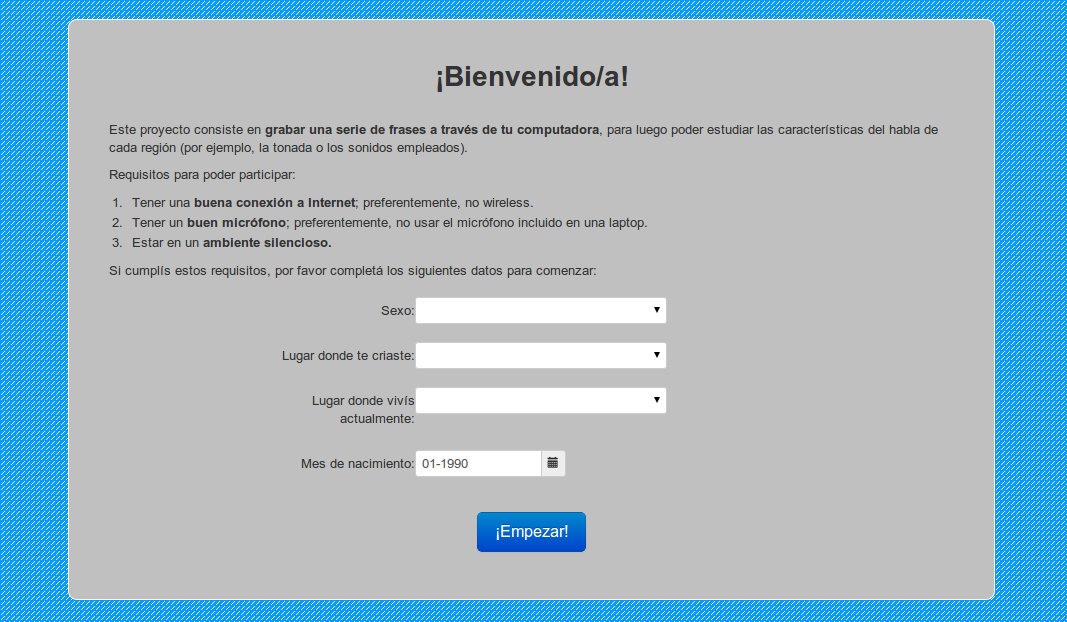
\includegraphics[width=0.8\textwidth]{pag-inicio2} }
		\caption{Encuesta inicial del sistema}
		\label{figEncuesta}
	\end{figure}
\end{frame}

\begin{frame}
	\frametitle{Sistema de grabación online}
	
	\begin{figure}[h!]
		\centerline{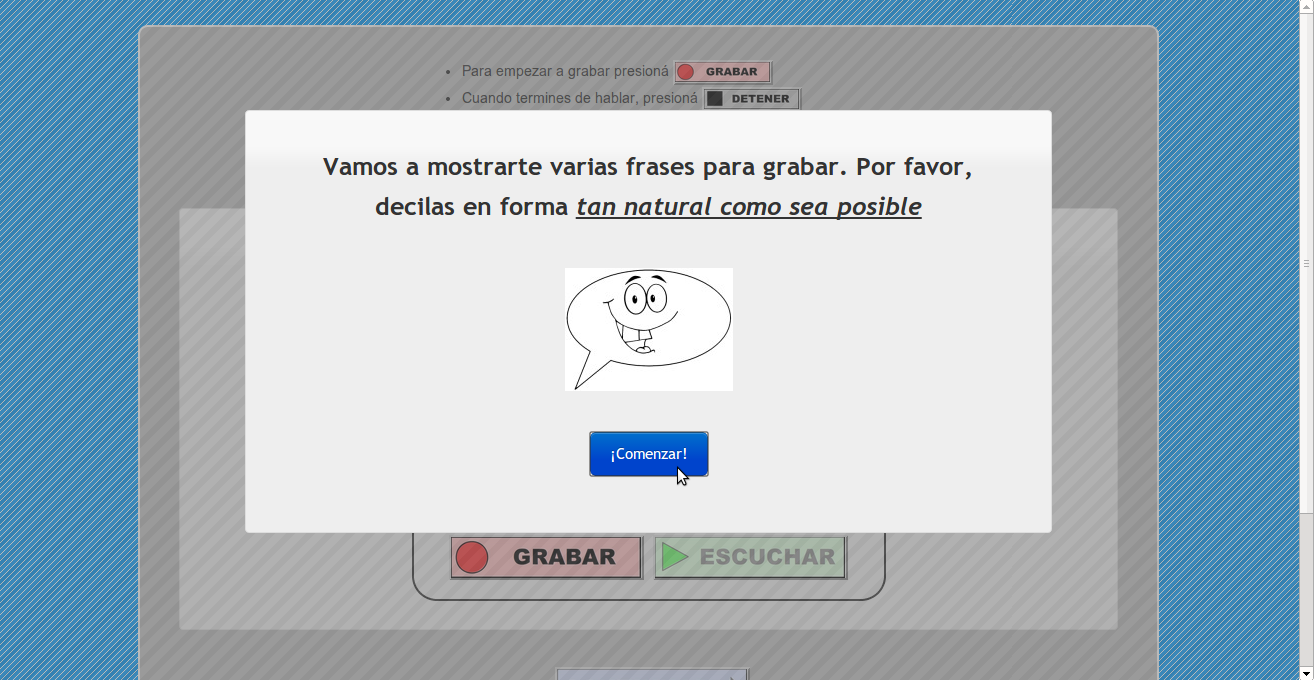
\includegraphics[width=0.8\textwidth]{pag-info2} }
		\caption{Instrucciones del experimento}
		\label{figInstrucciones}
	\end{figure}
\end{frame}

\begin{frame}
	\frametitle{Sistema de grabación online}
	
	\begin{figure}[h!]
		\centerline{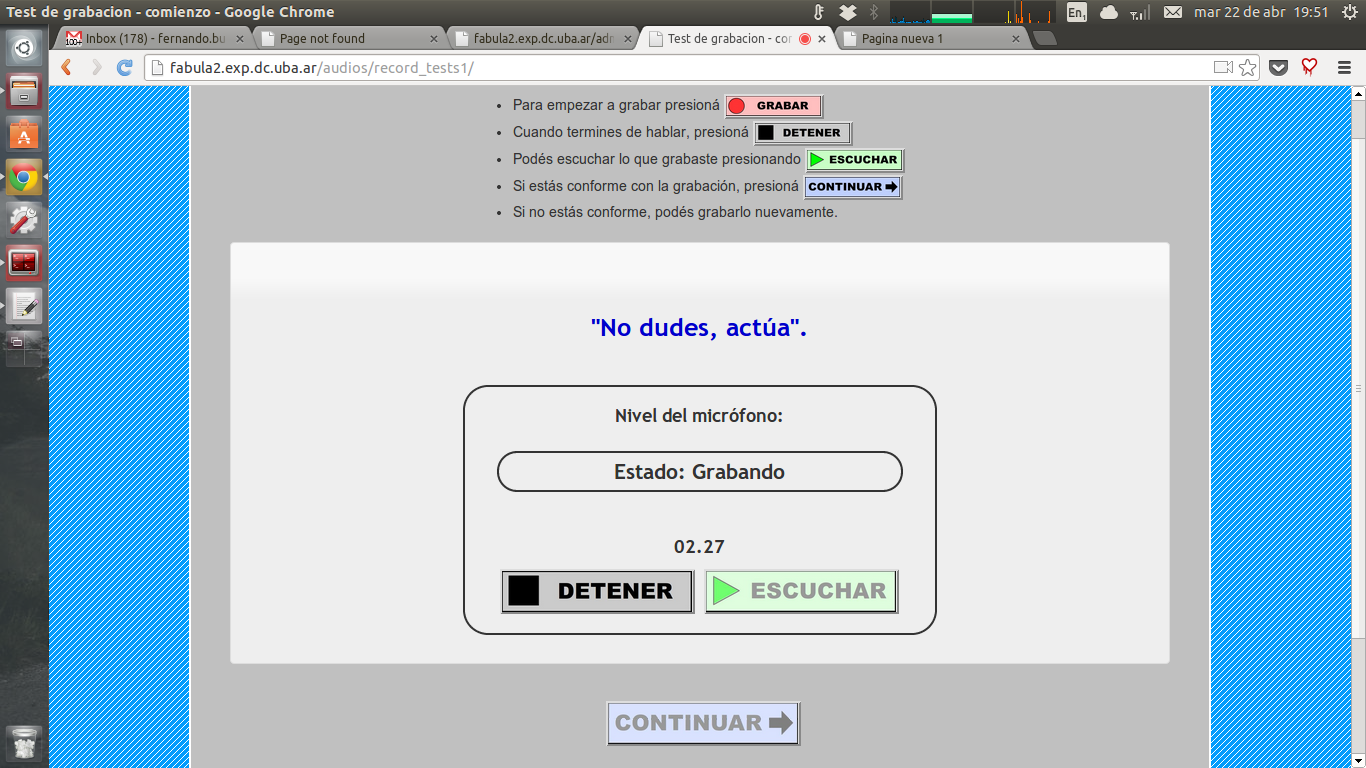
\includegraphics[width=0.8\textwidth]{pag-grabar1} }
		\caption{Grabando}
		\label{figEncuesta}
	\end{figure}
\end{frame}

\begin{frame}
	\frametitle{Sistema de grabación online}
	
	\begin{figure}[h!]
		\centerline{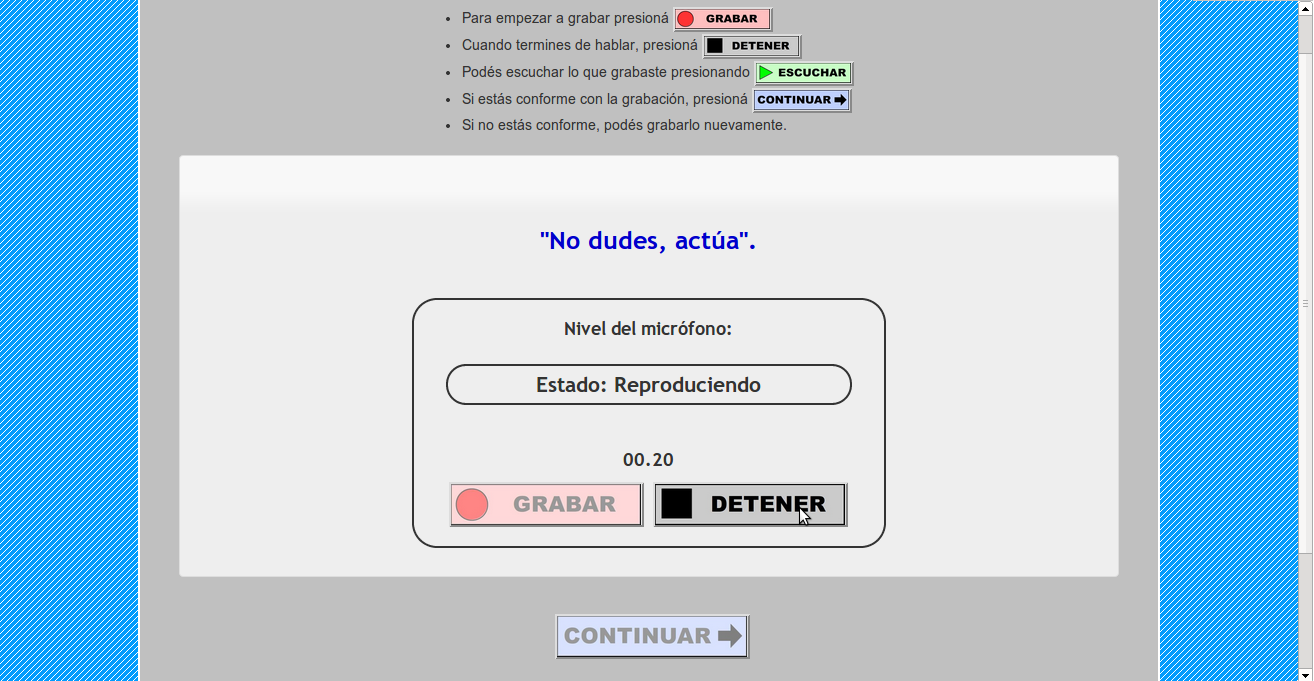
\includegraphics[width=0.8\textwidth]{pag-play1} }
		\caption{Reproduciendo}
		\label{figEncuesta}
	\end{figure}
\end{frame}

\section{Datos}

\begin{frame}
	\frametitle{Datos obtenidos}
	
	\begin{table}[h]
		\centering
		\begin{tabular}{|l|c|c|c|c|}
			\hline
			\textbf{}  & \textbf{Bs.As. } & \textbf{Cba.} & \textbf{Total} \\ \hline
			%\textbf{Conservar}  & 222 & 105 & 327 \\ \hline
			\textbf{Conservado}  & 220 & 90 & 310 \\ \hline
			\textbf{Problemas en el habla\footnote{Problemas más comunes: entonación exagerada y error al pronunciar una frase}}  & 33 & 15 & 48 \\ \hline
			\textbf{Mucho ruido de fondo}  & 2 & 12 & 14 \\ \hline
			\textbf{Sonido saturado}  & 2 & 0 & 2 \\ \hline
		\end{tabular}
		\caption{Evaluación manual de las grabaciones}
		\label{eva_table}
	\end{table}
	
	\begin{table}[H]
		\centering
		\begin{tabular}{|l|c|c|c|}
			\hline
			\textbf{}  & \textbf{Bs.As. } & \textbf{Cba.} & \textbf{Total} \\ \hline
			\textbf{Todos los intentos}  & 220 & 90 & 310 \\ \hline
			\cellcolor{blue!25}\textbf{Último intento}  & \cellcolor{blue!25}\textbf{181} & \cellcolor{blue!25}\textbf{79} & \cellcolor{blue!25}\textbf{260} \\ \hline
		\end{tabular}
		\caption{Cantidad de audios repetidos}
		\label{eva_table_rep}
	\end{table}
\end{frame}

\section{Extracción}

\begin{frame}
	\frametitle{Extracción de información}
	
	¿Cómo extraer atributos (features) de un audio?
	
	Etiquetamos el principio y el final de cada fonema.
	
	\begin{center}
			\textbf{ProsodyLab-Aligner: alineación forzada}
	\end{center}
	
	\begin{figure}[h!]
		\centerline{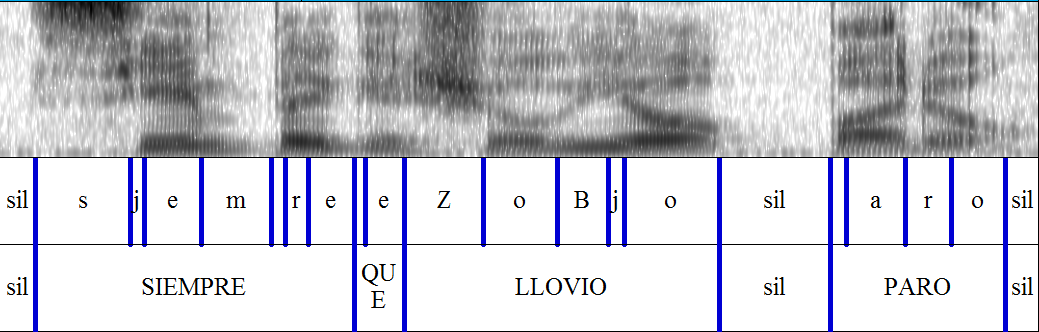
\includegraphics[width=0.9\textwidth]{frase-espectrograma-cortado2} }
	\end{figure}
\end{frame}

\begin{frame}
	\frametitle{Extracción de información}
	Definimos tipos de atributos:
	\begin{itemize}\itemsep=2ex
		\item Atributos acústicos
		\item Atributos fonéticos
		\item Atributos silábicos
	\end{itemize}
	{\tiny ProsodyLab, Python 2.7, Numpy, Pymatlab}
	
\end{frame}

%\begin{frame}
%	\frametitle{Extracción de información}
%	\begin{multicols}{2}
%		Definimos tipos de atributos:
%		\begin{itemize}
%			\item Atributo acústico
%			\item Atributo fonético
%			\item Atributo silábico
%		\end{itemize}
%		{\tiny ProsodyLab, Python 2.7, Numpy, Pymatlab}
%		
%		\begin{figure}[rh!]
%			\centerline{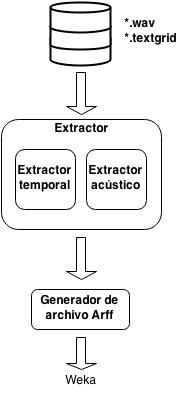
\includegraphics[width=0.25\textwidth]{diagrama_workflow} }
%		\end{figure}
%	\end{multicols}
%	
%\end{frame}

% Definicion para el timeline
\definecolor{mygreen}{RGB}{117,167,117}
\definecolor{myred}{RGB}{255,1,1}

\newcommand\myent[3]{%
	\footnotesize%
	$\begin{array}{@{}r@{}} 
	#1 \\ #2 \\#3
	\end{array}$%
}
\tikzset{
	every picture/.append style={
		execute at begin picture={\deactivatequoting},
		execute at end picture={\activatequoting}
	}
}
%fin timeline

\newcommand{\mfccvec}[3]% x, y
{  
	\node[fill={rgb:black,1;white,2;white,3}, rounded corners, draw, inner sep=+0pt] at (#1,#2) {\tiny \begin{tabular}{c}
			Coef 1\\\hline
			Coef 2\\\hline
			Coef 3\\\hline
			...\\\hline
			Coef N\\
		\end{tabular}};
		\node at (#1, #2-1) {{\tiny #3}};
	}

\newcommand{\mfccvecmax}[3]% x, y
{  
	\node[fill={rgb:red,1;white,2;white,3}, rounded corners, draw, inner sep=+0pt] at (#1,#2) {\tiny \begin{tabular}{c}
			Max(T1.coef1, T2.coef1, ... , TM.coef1)\\\hline
			Max(T1.coef2, T2.coef2, ... , TM.coef2)\\\hline
			Max(T1.coef3, T2.coef3, ... , TM.coef3)\\\hline
			...\\\hline
			Max(T1.coefN, T2.coefN, ... , TM.coefN)\\
		\end{tabular}};
		\node at (#1, #2-1) {{\tiny #3}};
	}
	
\newcommand{\intervalo}[2]% x, y
{  
	\draw (#1,#2) -- (#1+0.8,#2);
	\draw (#1,#2-.1) -- (#1, #2+.1);
	\draw (#1+0.8,#2-.1) -- (#1+0.8, #2+.1);
	
	\draw (#1,#2) -- (#1+.1,#2+.05);
	\draw (#1,#2) -- (#1+.1,#2-.05);
	
	\draw (#1+0.8,#2) -- (#1+0.8-.1,#2+.05);
	\draw (#1+0.8,#2) -- (#1+0.8-.1,#2-.05);
}
	
	\begin{frame}
		\frametitle{Extracción de información}
		\Large {Atributos acústicos: MFCC}
		
		\begin{figure}[H]	
				\begin{tikzpicture} [samples=200, domain=0:5*360,yscale=0.9]
				
				\node[anchor=south west,inner sep=0] (image) at (-0.6,1) {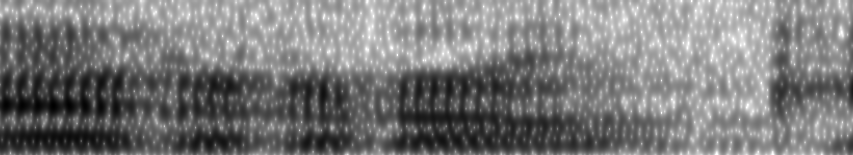
\includegraphics[width=0.9\textwidth]{perro-espectrograma-cortado.png}};
				
%				\begin{axis}[
%				width=12cm, height=4cm,
%				enlarge x limits=false,
%				xtick=\empty,
%				axis lines*=middle,
%				hide y axis
%				]
%				\addplot [no markers, smooth] {sin(x)+rand*2};
%				\end{axis}
				
				\def \posy {0};
				
				%flecha tiempo
				\draw [->] (8.5,-0.5+\posy) -- (9.5,-0.5+\posy);
				\node [align=center,below] at (9,-0.5+\posy) {tiempo};
				
				%grilla fonetica
				\draw [->] (-0.6,0.5+\posy) -- (10.3,0.5+\posy);
				\draw (1.2,-.1+0.5+\posy) -- (1.2, .1+0.5+\posy);
				\node [align=center,below] at (0,1.2+\posy) {/e/};
				\draw (5.2,-.1+0.5+\posy) -- (5.2, .1+0.5+\posy);
				\node [align=center,below] at (3.2,1.2+\posy) {/r/};
				\draw (6.8,-.1+0.5+\posy) -- (6.8, .1+0.5+\posy);
				\node [align=center,below] at (6,1.2+\posy) {/o/};	
				\draw (9.6,-.1+0.5+\posy) -- (9.6, .1+0.5+\posy);
				\node [align=center,below] at (8.3,1.2+\posy) { };
				\node [align=center,below] at (9.5,1.2+\posy) {{\footnotesize /k/}};
				\draw (9.2,-.1+0.5+\posy) -- (9.2, .1+0.5+\posy);
				
				\pause
				
				%linea vertical
				\draw[dotted] (1.2,0.5+\posy) -- (1.2,-0.4+\posy);
				\draw[dotted] (5.2,0.5+\posy) -- (5.2,-1.2+\posy);
				
				%grilla
				\draw [->] (-0.6,0+\posy) -- (10.3,0+\posy);	
				\foreach \r in {-0.4,0,0.4,0.8,...,10.3}
				\draw (\r,-.1+\posy) -- (\r, .1+\posy);
				
				%ventanas
				\intervalo{1.2}{-0.4+\posy};
				\intervalo{1.6}{-0.6+\posy};
				\intervalo{2}{-0.8+\posy};
				\intervalo{2.4}{-1+\posy};
				\node at (3.8,-1.2+\posy) {.......};
				\intervalo{4.4}{-1.2+\posy};
				
				\pause
				
				\mfccvec{-0.5}{-2.5+\posy}{Trama T1};
				\draw[blue, thick,->] (1.2,-0.55+\posy) -- (-0.5,-1.8+\posy);
				
				\pause
				
				\mfccvec{0.8}{-2.5+\posy}{Trama T2};
				\draw[blue, thick,->] (1.6,-0.75+\posy) -- (0.8,-1.8+\posy);
				
				\pause
				
				\mfccvec{2.1}{-2.5+\posy}{Trama T3};
				\draw[blue, thick,->] (2,-0.95+\posy) -- (2,-1.8+\posy);
				
				\pause
				
				\mfccvec{3.4}{-2.5+\posy}{Trama T4};
				\draw[blue, thick,->] (2.8,-1.15+\posy) -- (3.4,-1.8+\posy);
				
				\pause
				
				\node at (4.2, -2.5+\posy) {...};
				\mfccvec{5}{-2.5+\posy}{Trama TM};
				\draw[blue, thick,->] (4.8,-1.35+\posy) -- (5,-1.8+\posy);
				
				\pause
				%resultado
				\mfccvecmax{9.2}{-2.5+\posy}{Resultado vector máximos}
				\draw[decorate,decoration={brace,amplitude=7pt}] (6,-1.8+\posy) -- (6,-3.5+\posy);
				
				\end{tikzpicture}
		\end{figure}
\end{frame}

\begin{frame}
	\frametitle{Extracción de información}
	\Large {Atributos fonéticos}
	
	\begin{itemize}
		\item Duración de 'kt'
		\item Duración de 'sc'
		\item Duración de 'll'
		\item Duración de 'rr'
		\item Duración de 's' final
		\item Duración de cada fonema
		\item Duración de cada vocal 
		\item Duración de cada consonante
	\end{itemize}
\end{frame}



\begin{frame}
	\frametitle{Extracción de información}
	\Large {Atributos silábicos}
		
	\begin{itemize}
		\item Duración de la sílaba acentuada
		\item Duración de la sílaba anterior a la acentuada
	\end{itemize}
\end{frame}

\section{Análisis}

\begin{frame}
	\frametitle{Análisis}
	
	\begin{center}
		\Large {¿Cómo podemos saber si teniendo en cuenta estos atributos podemos clasificar mejor a un cordobés?}
		
	\end{center}
	
	\pause
	
	Dividimos nuestros datos en dos conjuntos: \textcolor{red}{\textbf{Entrenamiento}} y \textcolor{blue}{\textbf{Testeo}}.
	
	\begin{itemize}
		\item Un \textbf{clasificador} se entrenará con los datos del conjunto de \textcolor{red}{\textbf{Entrenamiento}}
		\item Luego, intentará clasificar correctamente el conjunto de \textcolor{blue}{\textbf{Testeo}}
	\end{itemize}
	
	Realizamos varias configuraciones similares a ésta, variando los elementos del conjunto de Testeo \textit{(folds)}
	
	Esta técnica se llama \textbf{Cross-validation}.

\end{frame}

\begin{frame}
	\frametitle{Análisis}

	\Large {Clasificadores}
	\begin{itemize}
		\item Zero Rules
		\item RIPPER
		\item C4.5
		\item Support vector machine
		\item Naive Bayes
	\end{itemize}
	
	\Large {Cross-validations}
	\begin{itemize}
		\item Clasificación por muestra 
		\item Clasificación por hablante
	\end{itemize}
	
\end{frame}

\begin{frame}
	\frametitle{Clasificación por muestra}
	
	{\Large Hablantes: 19 Buenos Aires, 8 Córdoba}
	
	\begin{center}
		\mycirc[blue] Hablante para train \mycirc[red] Hablante para test
	\end{center}
	
	\begin{table}[H]
		\centering
		\begin{tabular}{cccccccccccc}
			& \multicolumn{11}{c}{\textit{Número de hablante}} \\
			& 1 & 2 & 3 & 4 & 5 & 6 & 7 & ... & 25 & 26 & 27 \\
			\hline \\
			Fold 1 &\mycirc[red] & \mycirc[blue] & \mycirc[blue]  & \mycirc[blue]  & \mycirc[blue]  & \mycirc[blue]  & \mycirc[blue] & ... & \mycirc[blue] & \mycirc[blue] & \mycirc[blue]  \\
			
			Fold 2 &\mycirc[blue] & \mycirc[red] & \mycirc[blue]  & \mycirc[blue]  & \mycirc[blue]  & \mycirc[blue]  & \mycirc[blue] & ... & \mycirc[blue] & \mycirc[blue] & \mycirc[blue]  \\
			
			Fold 3 &\mycirc[blue] & \mycirc[blue] & \mycirc[red]  & \mycirc[blue]  & \mycirc[blue]  & \mycirc[blue]  & \mycirc[blue] & ... & \mycirc[blue] & \mycirc[blue] & \mycirc[blue]  \\
			
			\multicolumn{11}{c}{\textit{...}}	\\
			
			Fold 27 &\mycirc[blue] & \mycirc[blue] & \mycirc[blue]  & \mycirc[blue]  & \mycirc[blue]  & \mycirc[blue]  & \mycirc[blue] & ... & \mycirc[blue] & \mycirc[blue] & \mycirc[red]   \\
			
		\end{tabular}
		\caption{Esquema de validación cruzada}
		\label{HPTDT_esq_cv}
	\end{table}
\end{frame}
	
\begin{frame}
	\frametitle{Clasificación por muestra}
	
	Veamos el clasificador Ripper para el fold 4. Este es el conjunto de reglas que generó:
	
	\begin{flushleft}
		\begin{itemize}
			\item $(FON\_rr\_norm <= -6.901) and (ACU\_AverageRR\_7 <= 11.23) => place=cba (18.0/3.0)$ \\
			\item $(FON\_ll\_norm <= -7.975) and (ACU\_AverageLL\_6 <= 4.308) => place=cba (15.0/0.0)$
			\item $else => place=bsas (222.0/49.0)$
		\end{itemize}
	\end{flushleft}
	
	\begin{table}[H]
		\centering
		\begin{tabular}{|l|c|c|c|c|c|c|}
			\hline
			\textbf{}  & \textbf{Zero Rule} & \textbf{Ripper} & \textbf{C4.5} & \textbf{SVM} & \textbf{NaiveBayes} \\ \hline
			%\textbf{Fold 1}  &  &  &  &  &  \\ \hline
			%\hline \hline
			\textbf{Promedio} & 70  & 69 & 70 & 71 & 71 \\ \hline
		\end{tabular}
		\caption{Clasificación correcta en porcentaje}
		\label{HPTDT_clas_xval_porHab}
	\end{table}
	
\end{frame}

\begin{frame}
	\frametitle{Clasificación por muestra}
	
	Detalles:
	
	\begin{itemize}
		\item C4.5 obtuvo la misma performance que Zero Rule y su árbol de decisión fue muy pobre  
		\item Zero Rule obtuvo una buena performance y algunos clasificadores no pudieron obtener provecho de los atributos
	\end{itemize}
	
	\pause
	
	\begin{center}
		¿Qué sucedería si colapsáramos los atributos por hablante \\ y equilibramos nuestros datos?
	\end{center}
	
\end{frame}

\begin{frame}
	\frametitle{Clasificación por hablante}
	
	%{\Large Hablantes equilibrados: 8 Buenos Aires, 8 Córdoba}
	{\Large Hablantes equilibrados: 9 Buenos Aires, 8 Córdoba}
	
	\begin{center}
		\mycirc[blue] Hablante para train \mycirc[red] Hablante para test
	\end{center}
	
	\begin{table}[H, scale=0.3]
		\centering
		\begin{tabular}{cccccccccccc}
			& \multicolumn{11}{c}{\textit{Número de hablante}} \\
			%& 1 & 2 & 3 & 4 & 5 & 6 & 7 & ... & 14 & 15 & 16 \\
			& 1 & 2 & 3 & 4 & 5 & 6 & 7 & ... & 15 & 16 & 17 \\
			\hline \\
			Fold 1 &\mycirc[red] & \mycirc[blue] & \mycirc[blue]  & \mycirc[blue]  & \mycirc[blue]  & \mycirc[blue]  & \mycirc[blue] & ... & \mycirc[blue] & \mycirc[blue] & \mycirc[blue]  \\
			
			Fold 2 &\mycirc[blue] & \mycirc[red] & \mycirc[blue]  & \mycirc[blue]  & \mycirc[blue]  & \mycirc[blue]  & \mycirc[blue] & ... & \mycirc[blue] & \mycirc[blue] & \mycirc[blue]  \\
			
			Fold 3 &\mycirc[blue] & \mycirc[blue] & \mycirc[red]  & \mycirc[blue]  & \mycirc[blue]  & \mycirc[blue]  & \mycirc[blue] & ... & \mycirc[blue] & \mycirc[blue] & \mycirc[blue]  \\
			
			\multicolumn{11}{c}{\textit{...}}	\\
			
			%Fold 16 &\mycirc[blue] & \mycirc[blue] & \mycirc[blue]  & \mycirc[blue]  & \mycirc[blue]  & \mycirc[blue]  & \mycirc[blue] & ... & \mycirc[blue] & \mycirc[blue] & \mycirc[red]   \\
			
			Fold 17 &\mycirc[blue] & \mycirc[blue] & \mycirc[blue]  & \mycirc[blue]  & \mycirc[blue]  & \mycirc[blue]  & \mycirc[blue] & ... & \mycirc[blue] & \mycirc[blue] & \mycirc[red]   \\
			
		\end{tabular}
		\caption{Esquema de cross-validation}
		\label{}
	\end{table}
\end{frame}

\begin{frame}
	\frametitle{Clasificación por hablante}
	
	Juntamos los atributos de cada hablante de la siguiente forma.
	
	\begin{table}[H]
		\centering
		\resizebox{7cm}{!} {
		\begin{tabular}{|l|l|ccccc|}
			\hline
			\multicolumn{2}{|l|}{Atributos} & A1 & A2 & A3 & ... & AN \\
			\hline 
			\textbf{Hablante 1} & \textbf{Audio1} & 1 & ? & 2 & & 2\\
			& \textbf{Audio2} & ? & ? & 1 & ... & ? \\
			& \textbf{Audio3} & 2 & ? & 3 & & ? \\
			\hline
			\textbf{Hablante 2} & \textbf{Audio1} & 1 & ? & ? & ... & ? \\
			& \textbf{Audio2} & 1 & 2 & ? & & ? \\
			\hline
		\end{tabular}
		}
		\caption{Datos original}
		\label{}
	\end{table}
	
	esto pasaría a:
	
	\begin{table}[H]
		\centering
		\resizebox{7cm}{!} {
		\begin{tabular}{|l|l|ccccc|}
			\hline
			\multicolumn{2}{|l|}{Atributos} & A1 & A2 & A3 & ... & AN \\
			\hline 
			\textbf{Hablante 1} & \textbf{Audio1} & \textbf{1.5} & \textbf{?} & \textbf{2} & ... & \textbf{2}\\
			\hline
			\textbf{Hablante 2} & \textbf{Audio1} & \textbf{1} & \textbf{2} & \textbf{?} & ... & \textbf{?} \\
			\hline
		\end{tabular}
		}
		\caption{Datos modificados}
		\label{}
	\end{table}
\end{frame}

\begin{frame}
	\frametitle{Clasificación por hablante}
%	
%	Veamos un árbol de decisión generado por C4.5. Este corresponde al fold 7. 
%	
%	\dirtree{%
%		.1 root.
%		.2 $FON\_vowel\_norm <= 7.221824$.
%		.3 $FON\_ll\_norm <= -24.007: cba (2.33/0.22)$.
%		.3 $FON\_ll\_norm > -24.007: bsas (18.67/0.89)$.
%		.2 $FON\_vowel\_norm > 7.221824: cba (5.0)$.
%	}
%	
	\begin{table}[H]
		\centering
		\begin{tabular}{|l|c|c|c|c|c|c|}
			\hline
			\textbf{}  & \textbf{ZeroR} & \textbf{RIPPER} & \textbf{C4.5} & \textbf{SVM}\footnote{Corriendo T-test obtenemos $p < 0.05$} & \textbf{NaiveBayes} \\ \hline
			%\textbf{Promedio} & 53.33 & 60 & 60 & 93.33 & 80  \\ 
			\textbf{Promedio} & 53 & 53 & 76 & 94 & 76  \\ 
			\hline
		\end{tabular}
		\caption{Clasificación correcta en porcentaje}
		\label{class_corr_en_pct}
	\end{table}
	
\end{frame}

%
%\begin{frame}
%	\frametitle{Dejando un hablante fuera promediando los atributos desconocidos}
%	
%	\begin{table}[H]
%		\centering
%		\resizebox{7cm}{!} {
%		\begin{tabular}{|l|l|ccccc|}
%			\hline
%			\multicolumn{2}{|l|}{Atributos} & A1 & A2 & A3 & ... & AN \\
%			\hline 
%			\textbf{Hablante 1} & \textbf{Audio1} & 1 & ? & 2 & & 2\\
%			& \textbf{Audio2} & ? & ? & 1 & ... & ? \\
%			& \textbf{Audio3} & 2 & ? & 3 & & ? \\
%			\hline
%			\textbf{Hablante 2} & \textbf{Audio1} & 1 & ? & ? & ... & ? \\
%			& \textbf{Audio2} & 1 & 2 & ? & & ? \\
%			\hline
%			\end{tabular}
%		}
%		\caption{Original}
%		\label{}
%		\end{table}
%		
%			
%		Se cambia a ...
%		
%		\begin{table}[H]
%			\centering
%			\resizebox{7cm}{!} {
%			\begin{tabular}{|l|l|ccccc|}
%				\hline
%				\multicolumn{2}{|l|}{Atributos} & A1 & A2 & A3 & ... & AN \\
%				\hline 
%				\textbf{Hablante 1} & \textbf{Audio1} & 1 & ? & 2 & & 2\\
%				& \textbf{Audio2} & \textbf{1.5} & ? & 1 & ... & \textbf{2} \\
%				& \textbf{Audio3} & 2 & ? & 3 & & \textbf{2} \\
%				\hline
%				\textbf{Hablante 2} & \textbf{Audio1} & 1 & \textbf{2} & ? & ... & ? \\
%				& \textbf{Audio2} & 1 & 2 & ? & & ? \\
%				\hline
%			\end{tabular}
%			}
%			\caption{Modificado}
%			\label{}
%		\end{table}
%\end{frame}
%	
%\begin{frame}
%	\frametitle{Dejando un hablante fuera promediando los atributos desconocidos}
%	
%	\begin{table}[H]
%		\centering
%		\begin{tabular}{|l|c|c|c|c|c|c|}
%			\hline
%			\textbf{}  & \textbf{ZeroR} & \textbf{RIPPER} & \textbf{C4.5} & \textbf{SVM} & \textbf{NaiveBayes} \\ \hline
%			\textbf{Promedio} & 50 & 72.44 & 73.48 & 77.19 & 74.62 \\ \hline
%		\end{tabular}
%		\caption{Clasificación correcta en porcentaje}
%		\label{class_corr_en_pct}
%	\end{table}	
%	
%	\begin{table}[H]
%		\centering
%		\begin{tabular}{|l|c|c|c|c|c|c|}
%			\hline
%			\textbf{}  & \textbf{Student Test} & \textbf{Wilcoxon Test} \\ \hline
%			\textbf{ZeroR y Ripper}  & 0.06537 & 0.1284 \\ \hline
%			\textbf{ZeroR y C4.5}  & 0.06156 &  0.1111 \\ \hline
%			\textbf{ZeroR y NaiveBayes}  & 0.03916 & 0.06111 \\ \hline
%			\textbf{ZeroR y SVM}  &  0.02936 & 0.03522 \\ \hline
%		\end{tabular}
%		\caption{Resultados de cada test representado en p-valor}
%		\label{res_tests_wilcoxon_student}
%	\end{table}
%		
%\end{frame}
%
%\begin{frame}
%	\frametitle{Dejando un hablante fuera promediando los atributos desconocidos}
%	
%	Matríz de confusión mejores
%	
%	\begin{table}[H]
%		\centering
%		\begin{tabular}{|c|c|c|}
%			\hline
%			Buenos Aires & Córdoba & \\ \hline
%			33 & 1 & Buenos Aires\\ \hline
%			0 & 0 & Córdoba\\ \hline
%		\end{tabular}
%	\end{table}
%\end{frame}

\begin{frame}
	\frametitle{Selección de atributos de forma automática}
		
	¿Cuál es la importancia relativa de cada atributo?	\\
	Medimos cuanta información aporta cada atributo utilizando el algoritmo InfoGain.
	\begin{table}[H]
		\centering
		\begin{tabular}{|c|l|c|c|c|c|c|}
			\hline
			\textbf{Ganancia de Información} & \textbf{Atributo} \\ \hline
			0.07231     & FON\_consonant\_norm \\ \hline
			0.07217     & FON\_vowel\_norm \\ \hline
			0.03963     & \textbf{SIL\_syllableAccent\_normhd }\\ \hline
			0.03963     & \textbf{SIL\_prevSyllableAccent\_normhd} \\ \hline
			0.02332     & FON\_ll\_norm \\ \hline
			0.02285     & FON\_Sfinal\_norm \\ \hline
			0.02226     & ACU\_MinLL\_1 \\ \hline
			0.02144     & ACU\_AverageLL\_1 \\ \hline
		\end{tabular}
		\caption{Resultados de InfoGain}
		\label{infogain-table}
	\end{table}
\end{frame}

\section{Conclusiones}

\begin{frame}
	\frametitle{Conclusiones y trabajo futuro}
	
	{\Large Conclusiones}
	
	\begin{itemize}
		\item Armamos una plataforma para la recolección de grabaciones
		\item Caso de estudio: diferencia entre habla de Cba. y BsAs.
		\item Características del conjunto de datos y cómo repercute en sus resultados 
	\end{itemize}
	
	\pause
	
	{\Large Trabajo futuro}
	
	\begin{itemize}
		\item Grabaciones chequeadas entre los hablantes
		
		\pause
		
		\item Desarrollo de varios filtros para evitar grabaciones con problemas
		
		\pause
		
		\item Realizar clasificación en vivo a través de una página web
		
		\pause
		
		\item Mejores modelos variando sus parámetros y nuevos atributos 
		
	\end{itemize}
\end{frame}

\begin{frame}
	\begin{center}
		{\Large ¿Preguntas?}
	\end{center}
\end{frame}

\newcounter{finalframe}
\setcounter{finalframe}{\value{framenumber}}

% % % % % % % % % % % % % % % % % % % % % % % % % % % % % % %
% Más detalles

\section{Más detalles}

\begin{frame}[noframenumbering]
	\begin{center}
		\textbf{Más detalles...}
	\end{center}
\end{frame}

\begin{frame}[noframenumbering]
 	\frametitle{Diferencias entre Córdoba y Buenos Aires}
 	
	\begin{itemize}\itemsep=3ex
		\item \textbf{Regla 1: Los hablantes de Córdoba estiran la sílaba anterior a la acentuada mientras los de Buenos Aires no lo hacen} \\ 
	\end{itemize}
		
	\begin{center}
		\textit{`Especta\textcolor{red}{\textbf{\textit{cu}}}\textcolor{blue}{lar}'}
	\end{center} 
	
	\tab{Sílaba acentuada en \textcolor{blue}{\textit{`-lar'}}} \\ 
	\tab{La sílaba anterior \textcolor{red}{\textit{`-cu-'}} se alarga para hablantes de Córdoba}
\end{frame}

\begin{frame}[noframenumbering]
	\frametitle{Diferencias entre Córdoba y Buenos Aires}
	\begin{itemize}\itemsep=3ex
		\item \textbf{Regla 2: Los hablantes de Córdoba aspiran y elisionan la /s/ al finalizar una palabra. Esto no sucede en Buenos Aires} \\ 
	\end{itemize}	
		
	\begin{center}
		\textit{`Pájaro\textcolor{red}{\textbf{\textit{s}}}'}
	\end{center} 
	
	\begin{center}
		/\textcolor{red}{\textbf{\textit{s}}}/ se acorta su duración en el hablante de Córdoba
	\end{center}
\end{frame}

\begin{frame}[noframenumbering]
 	\frametitle{Diferencias entre Córdoba y Buenos Aires}
 	\begin{itemize}\itemsep=3ex
		\item \textbf{Regla 3: Para hablantes de Córdoba, la /s/ antes de la /c/ o /t/ suenan más suaves que para hablantes de Buenos Aires} \\ 
	\end{itemize}
	 	
	\begin{center}
		\textit{`Mo\textcolor{red}{s}ca'}
	\end{center} 
	 	
	\begin{center}
			/\textcolor{red}{s}/ suena más suave para Córdoba que para Buenos Aires
	\end{center}
	\end{frame}

\begin{frame}[noframenumbering]
 	\frametitle{Diferencias entre Córdoba y Buenos Aires}
 	\begin{itemize}\itemsep=3ex
 		\item \textbf{Regla 4: La `c' antes de la `t' se pronuncia con menor frecuencia para hablantes de Córdoba que para hablantes de Buenos Aires} \\ 
	\end{itemize}
 	
 	\begin{center}
 		\textit{`Do\textcolor{red}{c}tor'}
 	\end{center} 
 	
 	\begin{center}
 		No debe sonar el fonema /\textcolor{red}{c}/
 	\end{center}
\end{frame}

\begin{frame}[noframenumbering]
	\frametitle{Diferencias entre Córdoba y Buenos Aires}
	\begin{itemize}\itemsep=3ex
		\item \textbf{Regla 5: Para hablantes cordobeces la `y’ y `ll’ se pasa a `i’. No sucede esto para Buenos Aires} \\ 
	\end{itemize}
		
	\begin{center}
		\textit{`\textcolor{red}{ll}uvia'}
	\end{center} 
		
	\begin{center}
		Palabras con el fonema /\textcolor{red}{y}/ o /\textcolor{red}{ll}/ se pronuncian /\textcolor{red}{j}/
	\end{center}
\end{frame}
 
\begin{frame}[noframenumbering]
	\frametitle{Diferencias entre Córdoba y Buenos Aires}
	\begin{itemize}\itemsep=3ex
		\item \textbf{Regla 6: En hablantes cordobeces la /r/ no vibra mientras que en Buenos Aires pasa lo contrario} \\ 
	\end{itemize}	
	
	\begin{center}
		\textit{`Espá\textcolor{red}{rr}ago'}
	\end{center} 
		
	\begin{center}
		Para Córdoba /\textcolor{red}{r}/ debe ser suave en comparación de Buenos Aires
	\end{center}
	
	{\tiny Bibliografía:
		\begin{itemize}
			\item El español en la Argentina y sus variedades regionales - María Beatriz Fontanella de Weinberg
			\item Español en la Argentina - Elena Vidal de Battini
		\end{itemize}}	
\end{frame}

\begin{frame}[noframenumbering]
	\frametitle{Diseño del experimento}
	
	\begin{figure}[H]
		\centering
		\begin{tikzpicture}
		\begin{axis}[
		width=8cm,
		height=6cm,
		title={Porcentaje del total de frases por regla},
		xlabel={Cantidad de grabaciones},
		ylabel={Porcentaje del total de frases},
		xmin=0, xmax=25,
		ymin=0, ymax=100,
		xtick={0,5,10,15,20,25,30},
		ytick={0, 25, 50, 75, 100},
		legend pos=south east,
		ymajorgrids=true,
		xmajorgrids=true,
		grid style=dashed
		] 
		
		\addplot [mark=times*, line width=0.5pt]
		coordinates {
			(0,0)(1, 0)(2, 5)(3, 11)(4, 17)(5, 17)(6, 23)(7, 29)(8, 35)(9, 41)(10, 41)(11, 47)(12, 52)(13, 52)(14, 52)(15,58)(16, 64)(17, 64)(18, 70)(19, 76)(20, 76)(21, 76)(22, 82)(23, 82)(24, 88)(25, 94)(26, 100)
		};\addlegendentry{Regla 2};
		
		\addplot [mark=times*, dash pattern=on 10pt off 5pt, line width=0.5pt]
		coordinates {
			(0,0)(1,0)(2,0)(3,25)(4,25)(5,25)(6,25)(7,25)(8,50)(9,50)(10,50)(11,50)(12,50)(13,75)(14,75)(15,75)(16,75)(17,75)(18,75)(19,75)(20,100)(21,100)(22,100)(23,100)(24,100)(25,100)(26,100)
		};\addlegendentry{Regla 3};
		
		\addplot [mark=times*, line width=2pt] 
		coordinates {
			(0,0)(1, 0)(2, 0)(3, 0)(4, 25)(5, 25)(6, 50)(7, 50)(8, 50)(9, 75)(10, 75)(11, 75)(12, 75)(13, 75)(14, 75)(15,75)(16, 75)(17, 75)(18, 75)(19, 75)(20, 75)(21, 100)(22, 100)(23, 100)(24,100)(25,100)(26, 100)
		};\addlegendentry{Regla 4};
		
		\addplot [mark=times*, dash pattern=on 10pt off 5pt, line width=2pt]
		coordinates {
			(0,0)(4,0)(5,50)(13,50)(14,100)(26,100) 
		};\addlegendentry{Regla 5};
		
		\addplot [mark=times*, dotted, line width=2pt] 
		coordinates {
			(0,0)(2,20)(6,20)(7,40)(9,40)(10,60)(16,60)(17,80)(22,80)(23,100) 
		};\addlegendentry{Regla 6};
		
		
		%%		Tarea	rule 2:	rule 3:	rule 4:	rule 5:	rule 6:
		%		1	0	0	0	0	0
		%		2	5	0	0	0	20
		%		3	11	25	0	0	20
		%		4	17	25	25	0	20
		%		5	17	25	25	50	20
		%		6	23	25	50	50	20
		%		7	29	25	50	50	40
		%		8	35	50	50	50	40
		%		9	41	50	75	50	40
		%		10	41	50	75	50	60
		%		11	47	50	75	50	60
		%		12	52	50	75	50	60
		%		13	52	75	75	50	60
		%		14	52	75	75	100	60
		%		15	58	75	75	100	60
		%		16	64	75	75	100	60
		%		17	64	75	75	100	80
		%		18	70	75	75	100	80
		%		19	76	75	75	100	80
		%		20	76	100	75	100	80
		%		21	76	100	100	100	80
		%		22	82	100	100	100	80
		%		23	82	100	100	100	100
		%		24	88	100	100	100	100
		%		25	94	100	100	100	100
		%		26	100	100	100	100	100
		
		\end{axis}
		\end{tikzpicture}
		\caption{Porcentaje del total de frases grabadas por cada regla}
		\label{figFracesTraza}
	\end{figure}
\end{frame}

\begin{frame}[noframenumbering]
	\frametitle{Sistema de grabación online}
	
	\begin{figure}[h!]
		\centerline{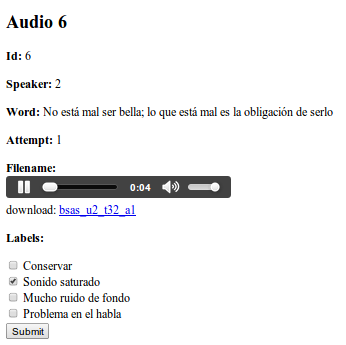
\includegraphics[width=0.6\textwidth]{categorizando_audios} }
		\caption{Administrador}
		\label{figEncuesta}
	\end{figure}
\end{frame}

\begin{frame}[noframenumbering]
	\frametitle{Extracción de información}
	\Large {Atributos acústicos: MFCC}
	
	{\normalsize \textbf{Escala Mel:} escala sobre la precepción auditiva humana
		
		\begin{enumerate}[(1)]
			\item Frame the signal into short frames.
			\item For each frame estimate the power spectrum (Fast Fourier Transform).
			\item Apply the mel filterbank to the power spectra, sum the energy in each filter.
			\item Take the logarithm of all filterbank energies.
			\item Take the DCT of the log filterbank energies. (DCT=discrete cosine transform)
			\item Keep DCT coefficients 2-13, discard the rest.
		\end{enumerate}
		
		Script en Matlab llamado por Pymatlab
		
	}
\end{frame}


\begin{frame}[noframenumbering]
	\frametitle{Extracción de información}
	\Large {Atributos fonéticos: cálculo duración de `kt’}
	
	\begin{center}
		{\textbf{\textit{``en la pelea se konose al soldaDo solo en la biktorja se konose al kaBaZero’’}}}
	\end{center}
	
	\begin{figure}[H]
		\centering
		\begin{tikzpicture}[xscale=0.5]
		\draw[x=2cm,step=0.05pt,thick,>=latex](0,0) -- (7.5,0);
		\foreach \Xc in {0,...,15}
		{
			\draw[thick] 
			(\Xc,0) -- ++(0,05pt);
		}
		\draw[dotted,thick] (-0.5,0) -- (0,0);
		\draw[dotted,thick] (15,0) -- (15.5,0);
		% la victoria se conoce
		\foreach \Xc/\Texto in 
		{5/k}
		{
			\fill[black] 
			([xshift=2pt]\Xc,0.05)  
			rectangle node[above] {\strut\small\Texto} 
			([xshift=-2pt]\Xc+1,0.15);  
		}
		\foreach \Xc/\Texto in 
		{0/l,1/a,2/$sil$,3/b,4/i,6/t,7/o,8/r,9/j,10/a,11/$sil$,12/s, 13/e, 14/$sil$}
		{
			\node[above] at ([xshift=15pt]\Xc,0.05){\strut\small\Texto} ;
		}
		\end{tikzpicture}
	\end{figure}
	
	\normalsize 
	\hspace{1cm} \[\frac{ X - \mu }{ \sigma }\]
	
	\begin{itemize}
		\item $X$ es el valor a normalizar (por ej.: la duración de un fonema dado).
		\item $\mu$ es el promedio de duración de la unidad utilizada en la grabación.
		\item $\sigma$ es el desvío estándar de la unidad utilizada en la grabación.
	\end{itemize}
	
\end{frame}


\begin{frame}[noframenumbering]
	\frametitle{Extracción de información}
	\Large {Atributos silábicos: sílaba anterior a la acentuada}
	
	\begin{center}
		{\textbf{\textit{``en la pelea se konose al soldaDo solo en la biktorja se konose al kaBaZero’’}}}
	\end{center}
	
	\begin{figure}[H]
		\centering
		\begin{tikzpicture}[xscale=0.7]
		\draw[x=2cm,step=0.05cm,thick,>=latex](0,0) -- (7.5,0);
		\foreach \Xc in {0,...,15}
		{
			\draw[thick] 
			(\Xc,0) -- ++(0,05pt);
		}
		\draw[dotted,thick] (-0.5,0) -- (0,0);
		\draw[dotted,thick] (15,0) -- (15.5,0);
		% la victoria se conoce
		\foreach \Xc/\Texto in 
		{2/bik,8/ko}
		{
			\fill[black] 
			([xshift=2pt]\Xc,0.05)  
			rectangle node[above] {\strut\small\Texto} 
			([xshift=-2pt]\Xc+1,0.15);  
		}
		\foreach \Xc/\Texto in 
		{0/la,1/$sil$,3/to*,4/rja,5/$sil$,6/se,7/$sil$,9/no*,10/se,11/$sil$,12/al, 13/$sil$, 14/ka}
		{
			\node[above] at ([xshift=15pt]\Xc,0.05){\strut\small\Texto} ;
		}
		\end{tikzpicture}
	\end{figure}
	
	\normalsize 
	\hspace{1cm} \[\frac{ X - \mu }{ \sigma }\]
	
	\begin{itemize}
		\item $X$ es el valor a normalizar (por ej.: la duración de un fonema dado).
		\item $\mu$ es el promedio de duración de la unidad utilizada en la grabación.
		\item $\sigma$ es el desvío estándar de la unidad utilizada en la grabación.
	\end{itemize}
	
\end{frame}

\begin{frame}[noframenumbering]
	\frametitle{Clasificación por muestra}
		
	\begin{center}
		\begin{tikzpicture}
		
		\begin{axis}[
		title={\textbf{Cantidad de grabaciones en cada grupo de Testeo}},
		xlabel={Folds},
		ylabel={Cantidad de grabaciones},
		scale only axis,
		width=4in,
		height=2in,
		xmin=0, xmax=28,
		ymin=0, ymax=45,
		axis on top]
		\addplot[
		ybar,
		fill=blue!15,
		bar width=0.102874in, 
		bar shift=0in,
		draw=black] 
		plot coordinates{ 
			(1, 10)(2, 5)(3, 11)(4, 1)(5, 11)(6, 5)(7, 5)(8, 5)(9, 10)(10,10)(11,2)(12,1)(13,1)(14,1)(15,10)(16,11)(17,2)(18,34)(19,18)(20,10)(21,40)(22,5)(23,15)(24,3)(25,11)(26,11)(27,11) 
		};
		
		\end{axis}
		\end{tikzpicture}	
	\end{center}
		
\end{frame}

\begin{frame}[noframenumbering]
	\frametitle{Clasificación por muestra}
	
	\textbf{Promedio de porcentaje correcto en cada fold:}
	\[
	{ \sum_{i=1}^{\text{\# de folds}} \text{Porcentaje instancias correctas en fold \textit{i}}
	\over
	\text{\# de folds}
	}
	\]
	
{\small 	\begin{table}[H]
		\centering
		\begin{tabular}{|l|c|c|c|c|c|c|}
			\hline
			\textbf{}  & \textbf{Zero Rule} & \textbf{Ripper} & \textbf{C4.5} & \textbf{SVM} & \textbf{NaiveBayes} \\ \hline
			%\textbf{Fold 1}  &  &  &  &  &  \\ \hline
			%\hline \hline
			\textbf{Promedio} & 70  & 69 & 70 & 71 & 71 \\ \hline
		\end{tabular}
		\caption{Clasificación correcta en porcentaje}
		\label{HPTDT_clas_xval_porHab}
	\end{table}}
	
	\textbf{Promedio de instancias correctas sobre instancias totales:}
	\small
	\[
	{ \sum_{i=1}^{\text{\# de folds}} \text{Cantidad de instancias correctas en fold \textit{i}}
		\over
		\text{\# de instancias}
	}
	\]

{\small 	\begin{table}[H]
		\centering
		\begin{tabular}{|l|c|c|c|c|c|c|}
			\hline
			\textbf{}  & \textbf{Zero Rule} & \textbf{Ripper} & \textbf{C4.5} & \textbf{SVM} & \textbf{NaiveBayes} \\ \hline
			%\textbf{Fold 1}  &  &  &  &  &  \\ \hline
			%\hline \hline
			\textbf{Promedio} & 69  & 63 & 69 & 70 & 65 \\ \hline
		\end{tabular}
		\caption{Clasificación correcta en cantidad de instancias}
		\label{HPTDT_clas_xval_porHab}
	\end{table}}
	
\end{frame}

\begin{frame}[noframenumbering]
	\frametitle{Clasificación por muestra}
	
	Árbol de decisión generado por C4.5 para cualquier fold para clasificación por muestra.
	
	\dirtree{%
		.1 root.
		.2 $bsas (249.0/68.0)$.
	}
	
\end{frame}

\begin{frame}[noframenumbering]
	\frametitle{Clasificación por hablante}
	
	Veamos un árbol de decisión generado por C4.5. Este corresponde al fold 7. 
	
	\dirtree{%
		.1 root.
		.2 $FON\_vowel\_norm <= 7.221824$.
		.3 $FON\_ll\_norm <= -24.007: cba (2.33/0.22)$.
		.3 $FON\_ll\_norm > -24.007: bsas (18.67/0.89)$.
		.2 $FON\_vowel\_norm > 7.221824: cba (5.0)$.
	}
		
\end{frame}

\begin{frame}[noframenumbering]
	\frametitle{Clasificación por hablante}
	
	Promediando los atributos por hablante \textbf{sin descartar datos} (utilizando los 27 hablantes)
	
	{\small 	
		\begin{table}[H]
			\centering
			\begin{tabular}{|l|c|c|c|c|c|c|}
				\hline
				\textbf{}  & \textbf{Zero Rule} & \textbf{Ripper} & \textbf{C4.5} & \textbf{SVM} & \textbf{NaiveBayes} \\ \hline
				\textbf{Promedio} & 70  & 77 & 70 & 96 & 88 \\ \hline
			\end{tabular}
			\caption{Clasificación correcta en porcentaje}
			\label{HPTDT_clas_xval_porHab}
		\end{table}
	}
	
	Promediando los atributos por hablante de los 17 hablantes
	(utilizando 9 de Buenos Aires, 8 Córdoba)
	
	{\small 	
		\begin{table}[H]
			\centering
			\begin{tabular}{|l|c|c|c|c|c|c|}
				\hline
				\textbf{}  & \textbf{Zero Rule} & \textbf{Ripper} & \textbf{C4.5} & \textbf{SVM} & \textbf{NaiveBayes} \\ \hline
				\textbf{Promedio} & 53  & 53 & 76 & 94 & 76 \\ \hline
			\end{tabular}
			\caption{Clasificación correcta en porcentaje}
			\label{HPTDT_clas_xval_porHab}
		\end{table}
	}
	
\end{frame}

\begin{frame}
	\frametitle{Clasificación por hablante}
	
	Detalles:
	
	\begin{itemize}
		\item Cada clasificación tiene 1 instancia para analizar \\
		Matrices de confusión muy pobres.
	\end{itemize}
	
	\begin{table}[H]
		\centering
		\begin{tabular}{|c|c|c|}
			\hline
			\multicolumn{2}{ |c| }{\textbf{Clasificadas como}} & \multirow{2}{*}{\textbf{Instancias de}}  \\ \cline{1-2}
			Buenos Aires & Córdoba &  \\ \hline
			1 & 0 & Buenos Aires\\ \hline
			0 & 0 & Córdoba\\ \hline
		\end{tabular}
	\end{table}
\end{frame}

\begin{frame}[noframenumbering]
	\frametitle{Selección de atributos de forma automática}
	
	Para cada atributo calcula la entropía de la clase y luego calcula la entropía\footnote{Cuán frecuente es una clase en una serie de muestras} de la misma sabiendo el valor de este atributo
	
	\begin{center}
		$InfoGain(Class,Attribute) = H(Class) - H(Class | Attribute)$
	\end{center}
	
	\begin{itemize}
		\item $H(Class)$ representa el valor de la entropía de la clase a predecir. Mide la incertidumbre asociada a la clase sin tener en cuenta el valor de ningún atributo en particular.
		\item $H(Class | Attribute)$ representa el valor de la entropía de la clase sabiendo el valor del atributo $Attribute$
	\end{itemize}
\end{frame}

\setcounter{framenumber}{\value{finalframe}}

\end{document}